%\documentclass{article}
%\usepackage[utf8]{inputenc}
%\usepackage{amsmath}
%\usepackage{natbib}
%\usepackage{graphicx}
%\usepackage{astrojournals} % Necesario para nombres de revistas en luis-ref.bib
%\usepackage[spanish, es-minimal]{babel}
%\usepackage{longtable}
%\usepackage{geometry}
%\usepackage{multirow, array}
%\newlength\figwidth
%\bibliographystyle{apj}

%\title{Catalog of stationary bowshock arcs in the Orion Nebula}

%\author{
  %Alumno: Luis Angel Gutiérrez Soto\\
  %Tutor: Dr. William Henney
%}
%\begin{document}
%\maketitle

%\chapter{Conclusiones}
\label{chap:conclu}

\section{Conclusiones generales}
\label{sec:con-g}

En este trabajo hemos catalogado arcos de proa estacionarios en la Nebulosa de Orión, identificando y  midiendo  parámetros observacionales de 73 objetos (ver figura \ref{fig:images}) de los cuales 20 no han sido reportados previamente. Las distancias proyectadas de estos objetos varían desde \(0.1'\) hasta \(10'\). A pesar de que estos arcos son poco estudiados en la literatura, ofrecen la oportunidad de analizar y probar los flujos a gran escala de la nebulosa y los flujos a pequeña escala que se originan en las estrellas de baja masa pre-secuencia principal y en sus discos. Con las mediciones de los parámetros observacionales hemos determinado tamaños, formas, orientaciones y brillos de \ha{}, corregidos por la contaminación de \nii{} y por extinción, de todos los arcos registrados en este trabajo. Además a partir de estos datos hemos estimado parámetros físicos tales como la  densidad en la cáscara  delimitada por dos choques y los flujos de momento tanto interno como externo. La identificación de los objetos del catálogo y las respectivas mediciones de los parámetros observacionales se relizaron usando imágenes en el óptico del \textit{HST}.\\

A partir de las mediciones de los parámetros observacionales: radio de los choques, radio de curvatura y ancho de la cáscara, hemos encontrado que el radio de los choques depende muy poco de la distancia proyectada. Pero si hay una dependencia significativa de la forma de los arcos con la distancia. Los objetos situados a grandes distancias del Trapecio tienden a tener cáscaras más anchas y más abiertas que los que se encuentran en el interior de la nebulosa, como se puede ver en las figuras \ref{fig:thikness} y \ref{fig:radii-curvatures}. Esto puede deberse a que los arcos externo son visibles en los objetos más alejados del Trapecio, mientras que los objetos situados en el interior de la nebulosa (es el caso particular de los proplyds LV) manifiestan que su choque interno es el radiativo. Además la interacción con el flujo de champaña ligeramente supersónico en las afueras de la nebulosa provoca que el ángulo entre las alas del choque exterior con respecto a la discontinuidad de contacto sea muy significativo, a diferencia de los proplyds LV, en cuyo caso la interacción con el  viento rápido estelar hace que la cáscara esté muy próxima a la discontinuidad de contacto provocando que el ángulo de separación de las alas del arco sean más pequeñas. Por otra lado como se mencionó en el capítulo \ref{chap:results} los arcos más abiertos como es el caso de LL2 están asociados a jets perpendiculares que se originan en la estrella joven. A pesar de estas premisas no es claro aún el por qué de esta discrepancia en las formas de los objetos de nuestro catálogo. \\  

A simple vista podemos ver en las figuras \ref{fig:position-arc} y \ref{fig:position-arc-zoom} del capítulo \ref{chap:results} que las orientaciones de los ejes de simetría de los arcos siguen aproximadamente la dirección radial. Pero un análisis más detallado (ver figura \ref{fig:pos-angular}) nos muestra que hay un desplazamiento angular significativo de \(\approx 30^{\circ}\) del eje del choque con respecto a la dirección radial de la nebulosa. Con esto podemos concluir que aunque con estos resultados se puede argumentar que los flujos aproximadamente radiales, provenientes del núcleo de la nebulosa, dominan sobre los flujos turbulentos y desordenados, tenemos que hay una desviación sistemática de los ejes de los choques particularmente en el sur de la nebulosa, indicando que estos movimientos no son estrictamente radiales. Con las comparaciones de las distribuciones de las posiciones de los arcos de proa con respecto a las distribuciones de las estrellas y de los proplyds en el cúmulo de la Nebulosa de Orión (ver figura \ref{fig:bow-proplyd-star-ratios}) hemos encontrado que hay al menos tres poblaciones distintas de arcos de proa estacionarios, donde los miembros de las dos poblaciones situados en el interior de la nebulosa son proplyds, mientras que los objetos exteriores correspondiendo a la tercera población no lo son.\\      

Demostramos que la emisión de \ha{} del gas más caliente, calentado por los choques, es muy pequeña en comparación a la emisión de \ha{} de la cáscara, por tanto la emisión de la zona de enfriamiento se puede despreciar. También demostramos que la emisión de \ha{} de los arcos está dominada por el gas que está en equilibrio térmico a la misma temperatura de la nebulosa, es decir aproximadamente a \(10^{4}~\K\), con lo que hemos determinado la densidad y la presión térmica en la cáscara chocada usando los parámetros observacionales medidos previamente (radios, ancho de la cáscara y brillo de \ha{}). De estos resultados podemos decir que hay una tendencia de la densidad a ser menor a distancias mayores, este resultado concuerda con el comportamiento del gas en la nebulosa, puesto que estimaciones previas de la densidad en la nebulosa han mostrado que este parámetro decrece con la  distancia desde \thC{} \citep{Odell:2010, Mesa:2008}. Subsecuentemente con estos resultados y con la suposición de que la presión térmica en la cáscara es igual a las presiones hidrodinámicas de los flujos externos e internos determinamos el flujo de momento de estos dos flujos para cada arco de nuestra muestra.\\
  
En este orden de ideas, en la figura \ref{fig:pressure} del capítulo anterior, observamos que en los proplyds LV el flujo de momento externo de nuestros objetos coincide con el flujo de momento del viento de la estrella masiva \thC{}, mientras que a distancia mayores el flujo de momento externo de nuestros objetos es mayor que el flujo de momento del viento estelar. Esto nos lleva a concluir que los objetos de las poblaciones interiores de la nebulosa están siendo confinados por el flujo de momento del viento de la estrella masiva \thC{}, que es la que domina la emisión en el Trapecio, mientras que los arcos más alejados, a partir de una distancia proyectada de \(0.05\)~pc, requieren un flujo de momento que sea de 10 a 100 veces más grande que el flujo estelar de la estrella masiva para poder confinarlos. Tenemos que probablemente los objetos de la población externa de la nebulosa están interaccionando con el flujo transónico de champaña de gas ionizado proveniente del núcleo de la nebulosa.\\ 

\begin{figure}
  \centering
  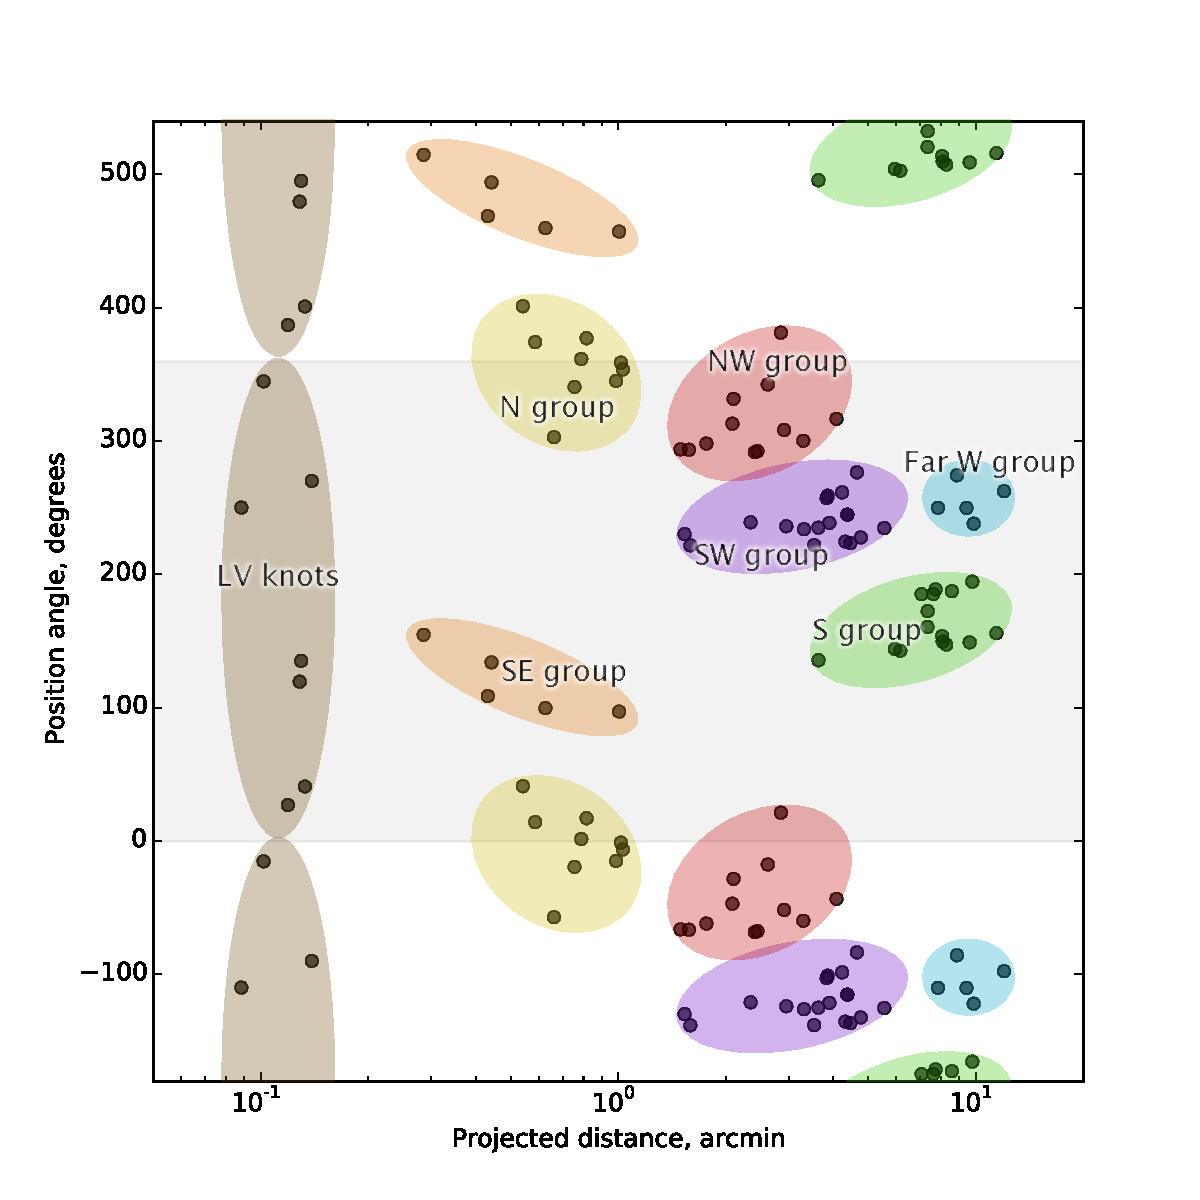
\includegraphics[width=\linewidth, clip]{arc-classify}
  \caption{Posición angular en el plano del cielo del eje de \thC{} a los choques de proa en función de la distancia proyectada. La región más oscura representa el rango angular que va desde \(0^{\circ}\) hasta \(360^{\circ}\) y las dos regiones sin sombra en la parte superior e inferior de la región sombreada, representan el mismo intervalo angular que la región con sombra. Las elipses de colores indican agrupaciones de objetos en las diferentes regiones de la nebulosa. }
 \label{fig:town}
\end{figure}

Con respecto a las estimaciones del flujo de momento interno hemos encontrado que para los arcos asociados a proplyds situados dentro de la distancia de \(0.2\)~pc desde el Trapecio, este flujo de momento interno no depende de la distancia. Los arcos más distantes de \(0.2\)~pc, de los cuales sólo la mitad están asociados a proplyds, muestran un flujo de momento interno que es \(\sim 10\) veces más débil, donde hay una tendencia de este flujo a ser más fuerte para los objetos que no son proplyds. Estos resultados son congruentes con la teoría que se ha realizado sobre el tema, puesto que los modelos predicen que el efecto de la radiación FUV sobre la fotoevaporación del disco es menos eficiente a distancias más grandes del Trapecio. Esto es una explicación del por qué el flujo de momento es más débil para los proplyds más alejados del Trapecio. Además en la figura \ref{fig:flow} se puede ver que los objetos que no son proplyds que pertenecen a la población de los objetos más alejados del Trapecio manifiestan fuertes vientos en comparación a los proplyds situados a las mismas distancias. Una explicación para esto consiste en que los discos de las estrellas T-Tauri pueden estar siendo fotoevaporados por la radiación de rayos-x provenientes de la cromósfera de las estrellas jóvenes. \\

\section{Trabajo a futuro}
\label{sec:future}

Algunos de los temas tratados en esta tesis que  serán explorados en posteriores trabajos, como por ejemplo:

\begin{itemize}
\item Estudiar y analizar el flujo suave y ligeramente supersónico de champaña proveniente del núcleo de la Nebulosa de Orión y su interacción con el viento estelar de las estrellas jóvenes. Estudiar la forma de los arcos de nuestros objetos que interaccionan con este flujo de champaña.
\item Verificar y estudiar de que manera los fuertes vientos presentes en los objetos LL y proplyds están relacionados con las estrellas más brillantes. Puesto que la figura \ref{fig:flow} del capítulo \ref{chap:theori}  nos muestra que hay una caída  en las tasa de pérdida de masa a partir de aproximadamente 1 arcmin de distancia desde \thC{}, esto quiere decir que hay una categorización de acuerdo a la diferencia de flujo de momento entre los objetos dentro y fuera de la nebulosa.   
\item La figura \ref{fig:town} nos muestra que los objetos de nuestros catálagos están divididos en 6 grupos de acuerdo su posición en la nebulosaa y su posición angular con respecto a \thC{} en el plano del cielo. Se realizará un estudio más detallado de estos grupos.
\end{itemize} 

%\end{document}